\documentclass[tikz]{standalone}
\usepackage{booktabs}
\usepackage{times}
\usepackage{sourcecodepro}

\usetikzlibrary{arrows.meta, decorations.pathreplacing, positioning}
\tikzset{
  na/.style = {baseline=-.5ex},
  every picture/.append style={remember picture},
  every node/.append style={font=\footnotesize},
}

\begin{document}
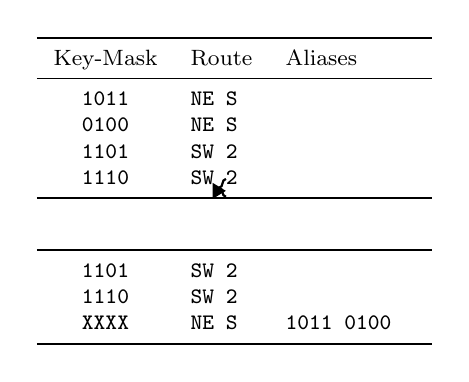
\begin{tikzpicture}
  % Original table
  \node (original) {
    \begin{tabular}{c l l}
      \toprule
      Key-Mask & Route & Aliases \\
      \midrule
      \tikz[na]\node [coordinate] (e0) {};\texttt{1011} & \texttt{NE S} \\
      \tikz[na]\node [coordinate] (e1) {};\texttt{0100} & \texttt{NE S} \\
      \texttt{1101} & \texttt{SW 2} \\
      \texttt{1110} & \texttt{SW 2} & \texttt{\hspace*{5.5em}}\\
      \bottomrule
      \vspace{1em}\\
      \toprule
      \texttt{1101} & \texttt{SW 2} \\
      \texttt{1110} & \texttt{SW 2} \\
      \tikz[na]\node [coordinate] (e2) {};\texttt{XXXX} & \texttt{NE S} & \texttt{1011 0100}\\
      \bottomrule
    \end{tabular}
  };

  % Add some arrows
  \draw [thick, decoration={brace}, decorate] ([xshift=-3pt, yshift=-.5ex] e1) --
                                              ([xshift=-3pt, yshift=+1ex] e0)
    node [midway, coordinate] (merge) {};
  \draw [thick, out=180, in=180, arrows={-Triangle[]}, shorten >=3pt] ([xshift=-2pt] merge) to (e2);
\end{tikzpicture}
\end{document}
